\documentclass[10pt,a4paper,oneside]{article}

\usepackage{listings}
\usepackage{color}

\definecolor{codegreen}{rgb}{0,0.6,0}
\definecolor{codegray}{rgb}{0.5,0.5,0.5}
\definecolor{codepurple}{rgb}{0.58,0,0.82}
\definecolor{backcolour}{rgb}{0.95,0.95,0.92}
 
\lstdefinestyle{mystyle}{
    backgroundcolor=\color{backcolour},   
    commentstyle=\color{codegreen},
    keywordstyle=\color{magenta},
    numberstyle=\tiny\color{codegray},
    stringstyle=\color{codepurple},
    basicstyle=\footnotesize,
    breakatwhitespace=false,         
    breaklines=true,                 
    captionpos=b,                    
    keepspaces=true,                 
    numbers=left,                    
    numbersep=5pt,                  
    showspaces=false,                
    showstringspaces=false,
    showtabs=false,                  
    tabsize=2
}
 
\lstset{style=mystyle}


\usepackage[utf8]{inputenc}
\usepackage{verbatim}
\usepackage[T1]{fontenc}
\usepackage{amsmath}
\usepackage{amsfonts}
\usepackage{amssymb}
\usepackage{graphicx}
\usepackage[left=2cm,right=2cm,top=2cm,bottom=2cm]{geometry}
\usepackage{multicol}
\usepackage{amsthm}
\author{Baptiste Chanus}

\title{Anticipating applications failures in containerized, micro-service and cloud architectures using AI}

\begin{document}

\begin{center}
\begin{Huge}
White Paper
\end{Huge}
\vspace{0.8cm}

\begin{Large}
Anticipating applications failures in containerized, micro-service and cloud architectures using AI
\end{Large}
\end{center}

\vspace{0.8cm}

\begin{figure}[h!]
\centering
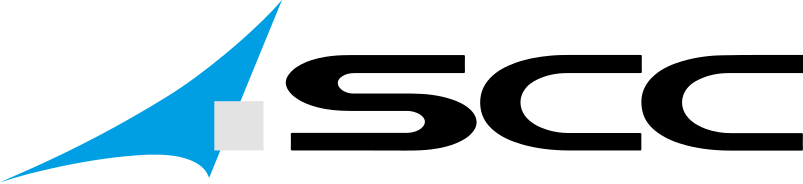
\includegraphics[scale=0.5]{./images/PNG/scc-logo.png}
\end{figure}

\vspace{0.8cm}

\begin{abstract}
	Throughout the whole industry many systems relies on clouds, network, Datacenter and software components stabilities. Thus, each application has to be available most of the time. In addition, the IT governance model pressure IT teams to take strong commitments (KPI) of accountability to address the outages as fast as possible. This work is about a learning algorithm whose goal is to give a hint on when an unavailability is going to occurs. In cooperation with monitoring systems used to collect the data on applications availability, like a nagios based softwares, the algorithm's aims to process data by gathering few different classical techniques, such as neural network genetic algorithm. This method is however somehow based on empirical thoughts and target at guessing a failure before it happens.
\end{abstract}

\vspace{1.2cm}

\begin{multicols}{2}
\section{Introduction}
Contracted applications run within a maximum amount of time of unavailability per day. Thus when an incident occurs a race against time begins. The issue has to be diagnosed and fixed as fast as possible because this time is taken on the whole unavailability time. This amount of time is one of the most important key performance indicator (KPI) of an service level aggreement (SLA) contracted by indrustry class IT services. We try to find a solution that could help anticipating these problems so the resolution time is the shorter possible.
\\
When in 2017 we tried to find a solution to the problem, we decided to use the log files of Nagios based monitoring systems we had access to. Our thougth was that we could establish a learning process using only the nagios disponibility data (which is described in the following part) to predict any failure of the application. The whole initial solution is explained in details throughout the first part but is build upon the assumption that the changes in the structure of the application are scarce which was a coherent assumption by this time.
\\ However technologies have evolved and applications may have small changes in their structure on a regular basis which make any form of learning pretty difficult since the training is made with a specific structure of the application. This change in architecture are typically those expected with new kind of infrastructure like, as an example, the orchestrated containerized applications. This is why in a second part we'll focus on how to target specific hosts, those with the most influence on the application's state, so we can apply our previous learning method on a subset of all the hosts in the application that won't change too much. Finally we'll also try to regroup some of the hosts together in such a way that some may be added or remove only the group while be taken into account and the learning won't be affected by the structure changes.
\end{multicols}


\begin{multicols}{2}
\section{Availability based method}
This first method uses nagios disponibility data, which means we have access, for each host and service of the application, only to the disponibility score between 0 and 3 (0: OK, 1: Warning, 2: Critical, 3: Unknown) and not to the exact value of each parameter. We are going to use historical data from old logs to train an algorithm of machine learning combining two learning techniques which are neural networs and the principle of genetic algorithms that we'll then use on the live data to predict the outage of the application that will eventually occur. However as explain in the introduction this method has serious rigidity issues as the training is made on a specific application's structure we'll discuss this limit as a conclusion to this method.
\subsection{Application model}
The model for the application we chose is a tree of dependencies. The application is the root of the tree, the internal nodes are the hosts and the leaves are the services. To each node, a relationship is associated to its children. This logical gate indicates wether all of them are required for the availability of this node or if some can be down without making this node unavailable. These relationships are only the known ones, which means that they are explicit, they are obvious looking at the design of the application. We may have relationships that are implied by the interaction of the internal nodes that occurs in a real life system without us being aware of it, but they are not obvious during the creation process of the application. (see Figure~\ref{exampletree} below)
\end{multicols}

\vspace{0.8cm}

\begin{figure}
\centering
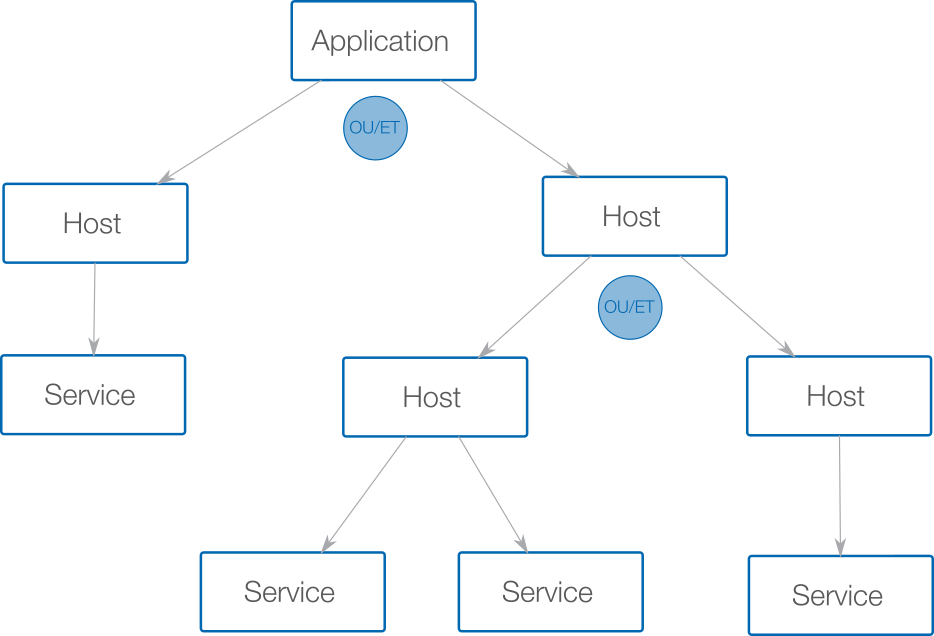
\includegraphics[scale=0.5]{./images/PNG/abrerelation.png}
\caption{Tree example}
\label{exampletree}
\end{figure}

\vspace{0.8cm}

\begin{multicols}{2}
We also define an image as the state of the whole application i.e. the state of all of its components (hosts and services) at a point in time. This is represented as an array where there are 4 rows, one for each state (0-3) and as many column as hosts and services. The state of an host or a service is given by a boolean in the array (true in the row that is the corresponding state and false everywhere else) illustrated on Figure~\ref{tab}

\end{multicols}

\vspace{0.8cm}

\begin{figure}[!h]
\centering
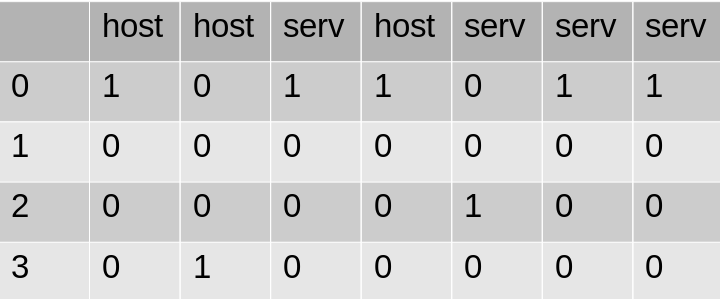
\includegraphics[scale=0.5]{./images/image.png}
\caption{General image}
\label{tab}
\end{figure}

\vspace{0.8cm}


\begin{multicols}{2}
\subsection{Processing data}
We are going to use supervised machine learning, therefore we need to label the historical data we'll use to train our neural network. The neural network will have to guess the amount of epoch remaining until the next outage, hence we have to extract from the log all the epochs where the application was unaivalable. This can be achieved with a request to the database in which are stored all the dates of the beginning and the ending of an outage and then, by taging the images whose epoch are in between a start and an end.
 In addition, we need to associate with each image the time remaining before the next outage. This can be done easily using what we calculated before.
\\We now compute a mean of all the image immediately preceding an outage. At this point, we made an assumption. We assumed that enough informations has been collected to feed the neural network and a raisonnably accurate guess would be stored in the comparison between an image and the mean we calculated. We are going to call this mean image the Reference.
\\The comparison between an image and the Reference is made by using a simple coordinate by coordinate distance i.e. noting $a_{i}$ the coordinates of the image and $r_{i}$ the ones of the Reference we use, for a given $k\in\mathbb{N}$, the following formula:

\vspace{0.8cm}

\begin{Large}
\[ d(a, r) = \sqrt[k]{\sum \mid{a_i - r_i}\mid^{k}} \]
\end{Large}

\vspace{0.8cm}

\subsection{Neural networks}
The first learning of the algorithm is via neural networks. We are going to train a neural network to guess how much time is remaining until the next outage. A network with a given structure is the set of its weights and biases which are the parameters we'll try to evolve during the learning process. They are going to be randomly initialized, this is why, before the training, our network can be summarize to its structure. So, we'll represent a network by two list of integers. One that will specify the input of the neural network and another for its hidden layers (we only need one output : the guess). The first list length is the total of inputs of the network and each integer in this list will be used as the $k$ in the distance formula thus each input will take a different value of a different comparison between the image and the reference. The second list length is the total number of hidden layer and the $i-th$ integer in the list is the amount of neurones in the layer $i$.
\end{multicols}

\vspace{0.8cm}

\begin{figure}[!ht]
\centering
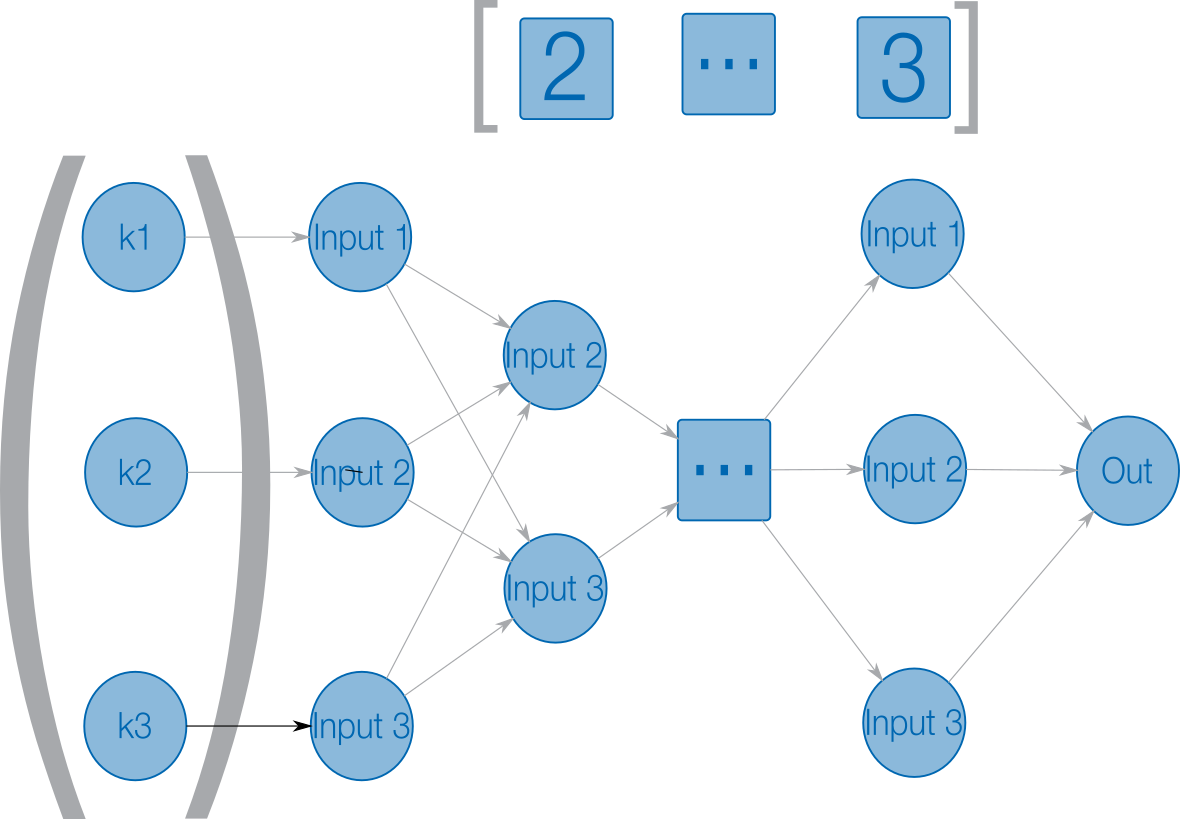
\includegraphics[scale=0.50]{./images/PNG/reseau.png}
\caption{Network structure}
\label{reseau}
\end{figure}

\vspace{0.8cm}

\begin{multicols}{2}
Once the network is defined we start the learning phase. We use our labelled data to train the network to guess the time until the next outage with the backpropagation algorithm. This classical algorithm do the computation with the labelled data, evaluate the cost i.e. the error made by the network between the result just obtained and the label associated with the data. Then, this cost is used to modify the weights and biases of the network.
The formula to reevaluate the weights $w^l$ and biases $b^l$ is (for the layer $l$):

\vspace{0.8cm}

\begin{Large}
\[ w^l \leftarrow  w^l-\frac{\eta}{m} \sum_x \delta^{x,l} \,{}^t(a^{x,l-1}) \]
\[ b^l \leftarrow b^l-\frac{\eta}{m} \sum_x \delta^{x,l} \]
\end{Large}

\vspace{0.8cm}


Where $\eta$ is the learning rate, which means a coefficient to control the speed of the changes made upon the weights and biases. $m$ is the number of element used to evaluate the changes that have to be made. $\delta$ is the error and $x$ is a piece of training data.
However several problems appears here. First, when we train the network we are minimizing a function of its inputs which is not convex. So, it has not necessarily only one global minimum, we can, for instance, switch two neurones on the same layer. As a consequence, it could converge only to a local minimum.
The second problem is that we have to determine a good set of hyperparameters i.e. the structure lists of the network, the learning rate and the size of the training data.

\subsection{Evolving hyperparameters}
The solution we proposed is a solution for both problem. It consists in applying the principle of genetic algorithm to our neural networks. After every application outage, we'll evaluate the performance of each network with a fitness function that takes into account the difference between the guess, the reality and its score on an evaluation set of historical data randomly selectionned. So with the distance $x\in\mathbb{R}^{+*}$ and the score $y\in[0, 1]$ we set the function fitness $f$ arbitrarily defined by :

\vspace{0.8cm}

\begin{Large}
\[ f(x, y) = y^{\frac{1}{50}+\frac{1}{1+e^{\frac{1}{1+x}}}} \]
\end{Large}

\vspace{0.8cm}

This function has only been chosen for its shape illustrated on Figure ~\ref{fonction}

\end{multicols}

\vspace{0.8cm}

\begin{figure}[!ht]
\centering
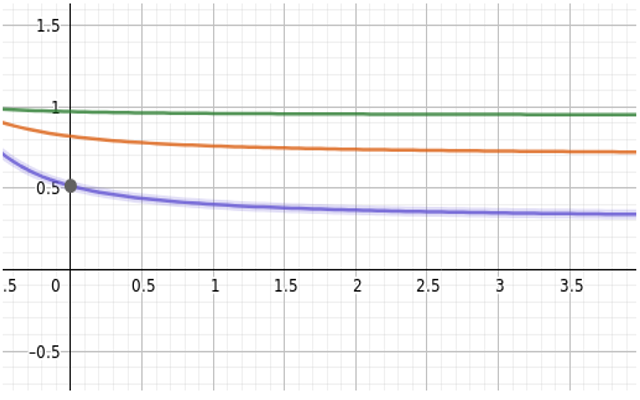
\includegraphics[scale=0.5]{./images/fitness.png}
\caption{Fitness evaluation for several values of y}
\label{fonction}
\end{figure}

\vspace{0.8cm}


\begin{multicols}{2}
At the beginning we create a population of multiple neural networks that we train separatly from different starting parameters (structure, weights and biases). During the analysis we can use the computation of all these networks. Because they started their training from different configurations they propably didn't converge to the same minimum of the function, thus we increase the probability of getting close to a global minimum. 
\\We use all the guesses from all of the networks in the population to get the amount of time we are trying to predict. Then after the application outage we apply the fitness function we introduced above to evaluate individualy the networks (Figure~\ref{pop}) and we generate the next generation using the ones with best results. To perform the selection we normalize all the score so that the total sum is $1$ and we randomly select some networks, the higher their score the higher the probability of being selected.
\end{multicols}

\vspace{0.8cm}

\begin{figure}[!ht]
\centering
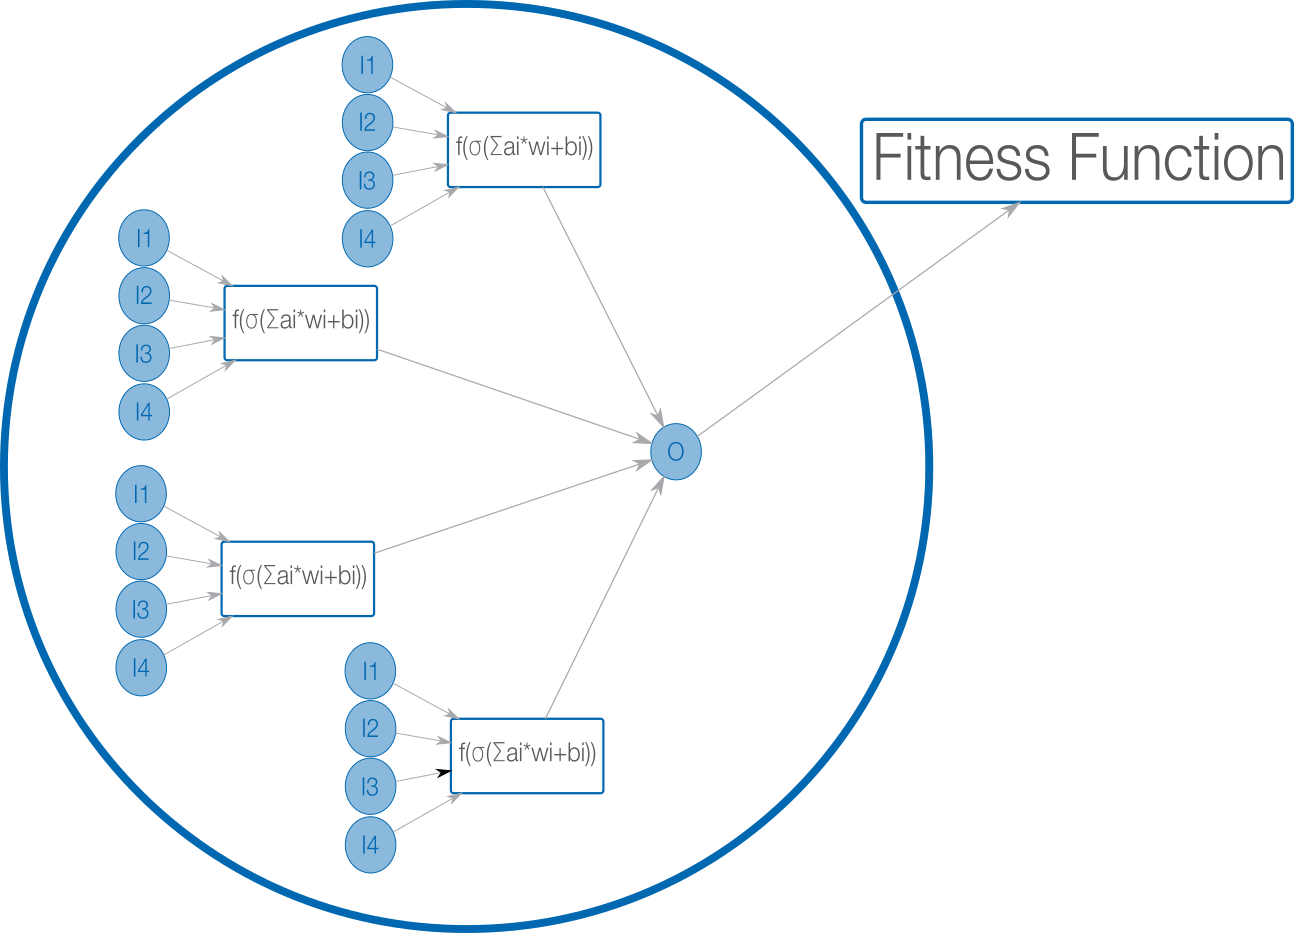
\includegraphics[scale=0.5]{./images/PNG/Population.png}
\caption{A population of network}
\label{pop}
\end{figure}

\vspace{0.8cm}

\begin{multicols}{2}
In the process we also add little mutations to the hyperparameters so that we have less chance of getting stuck in a non-optimal configuration. This method also solved the problem of choosing the set of hyperparameters because they are evolving throughout the execution of the algortihm.
With two given network another is created by generating an empty list we fill with elements of a list or the other with probability $\frac{1}{2}$. Then with a little probability called $mutation ~rate$ we introduce mutations which can be either a little variation of an integer in the lists or of the size of each list.


\subsection{Conclusion and limits}
This method can be pretty efficient because we can also collect data from past runs to determine the best structure to start the genetic principle with, which could be seen as another form of learning. However eventhough some part of it could be useful the full method is not feasible because it's unadapted to the new standard architectures of application. Indeed the whole process lies on the training of neural networks that was made using a specific architecture of the application and it shall not evolve during the execution of the algorithm for two big reasons. The first is that the learning would be, in the best case, far less efficient and the second problem is that the comparison is made coordinate by coordinate with an image calculated from historical data. Thus we couldn't compare new images with the old mean and the whole algorithm falls apart.

 
\\ \\This indicates a path to follow. We should find a way to identify which variables of the application are the most impactful. This is an interesting question because identifying these variable would not only making possible to restrain the number of data used to feed the neural network, but would allow to add new ones without directly breaking the whole training. Indeed, if the newly introduced variable is important the training could be done later without preventing the comparison. Furthermore, this would be a relevant information to help the diagnosis of an application. This is why the following part will focus on the identification of these variables. With this in mind analazing raw data will be more relevant hence we wont use the monitoring state data but directly values obtained from sensors. Therefore some new method of learning will eventually be explored.


\section{Raw data enhancements}
We need more adaptability because legacy applications weren't changing their achitecture often, they were designed following the Figure~\ref{omodl} schema. This model however didn't allow a lot of optimisations. Therefore now, to adapt to the demand, application are now based on a more horizontal or distributed model as illustrated on Figure~\ref{nmodl}. This cause the infrastructures of the application to change more often. This problem will be discussed in the following part.
\end{multicols}

\begin{figure}[!ht]
\centering
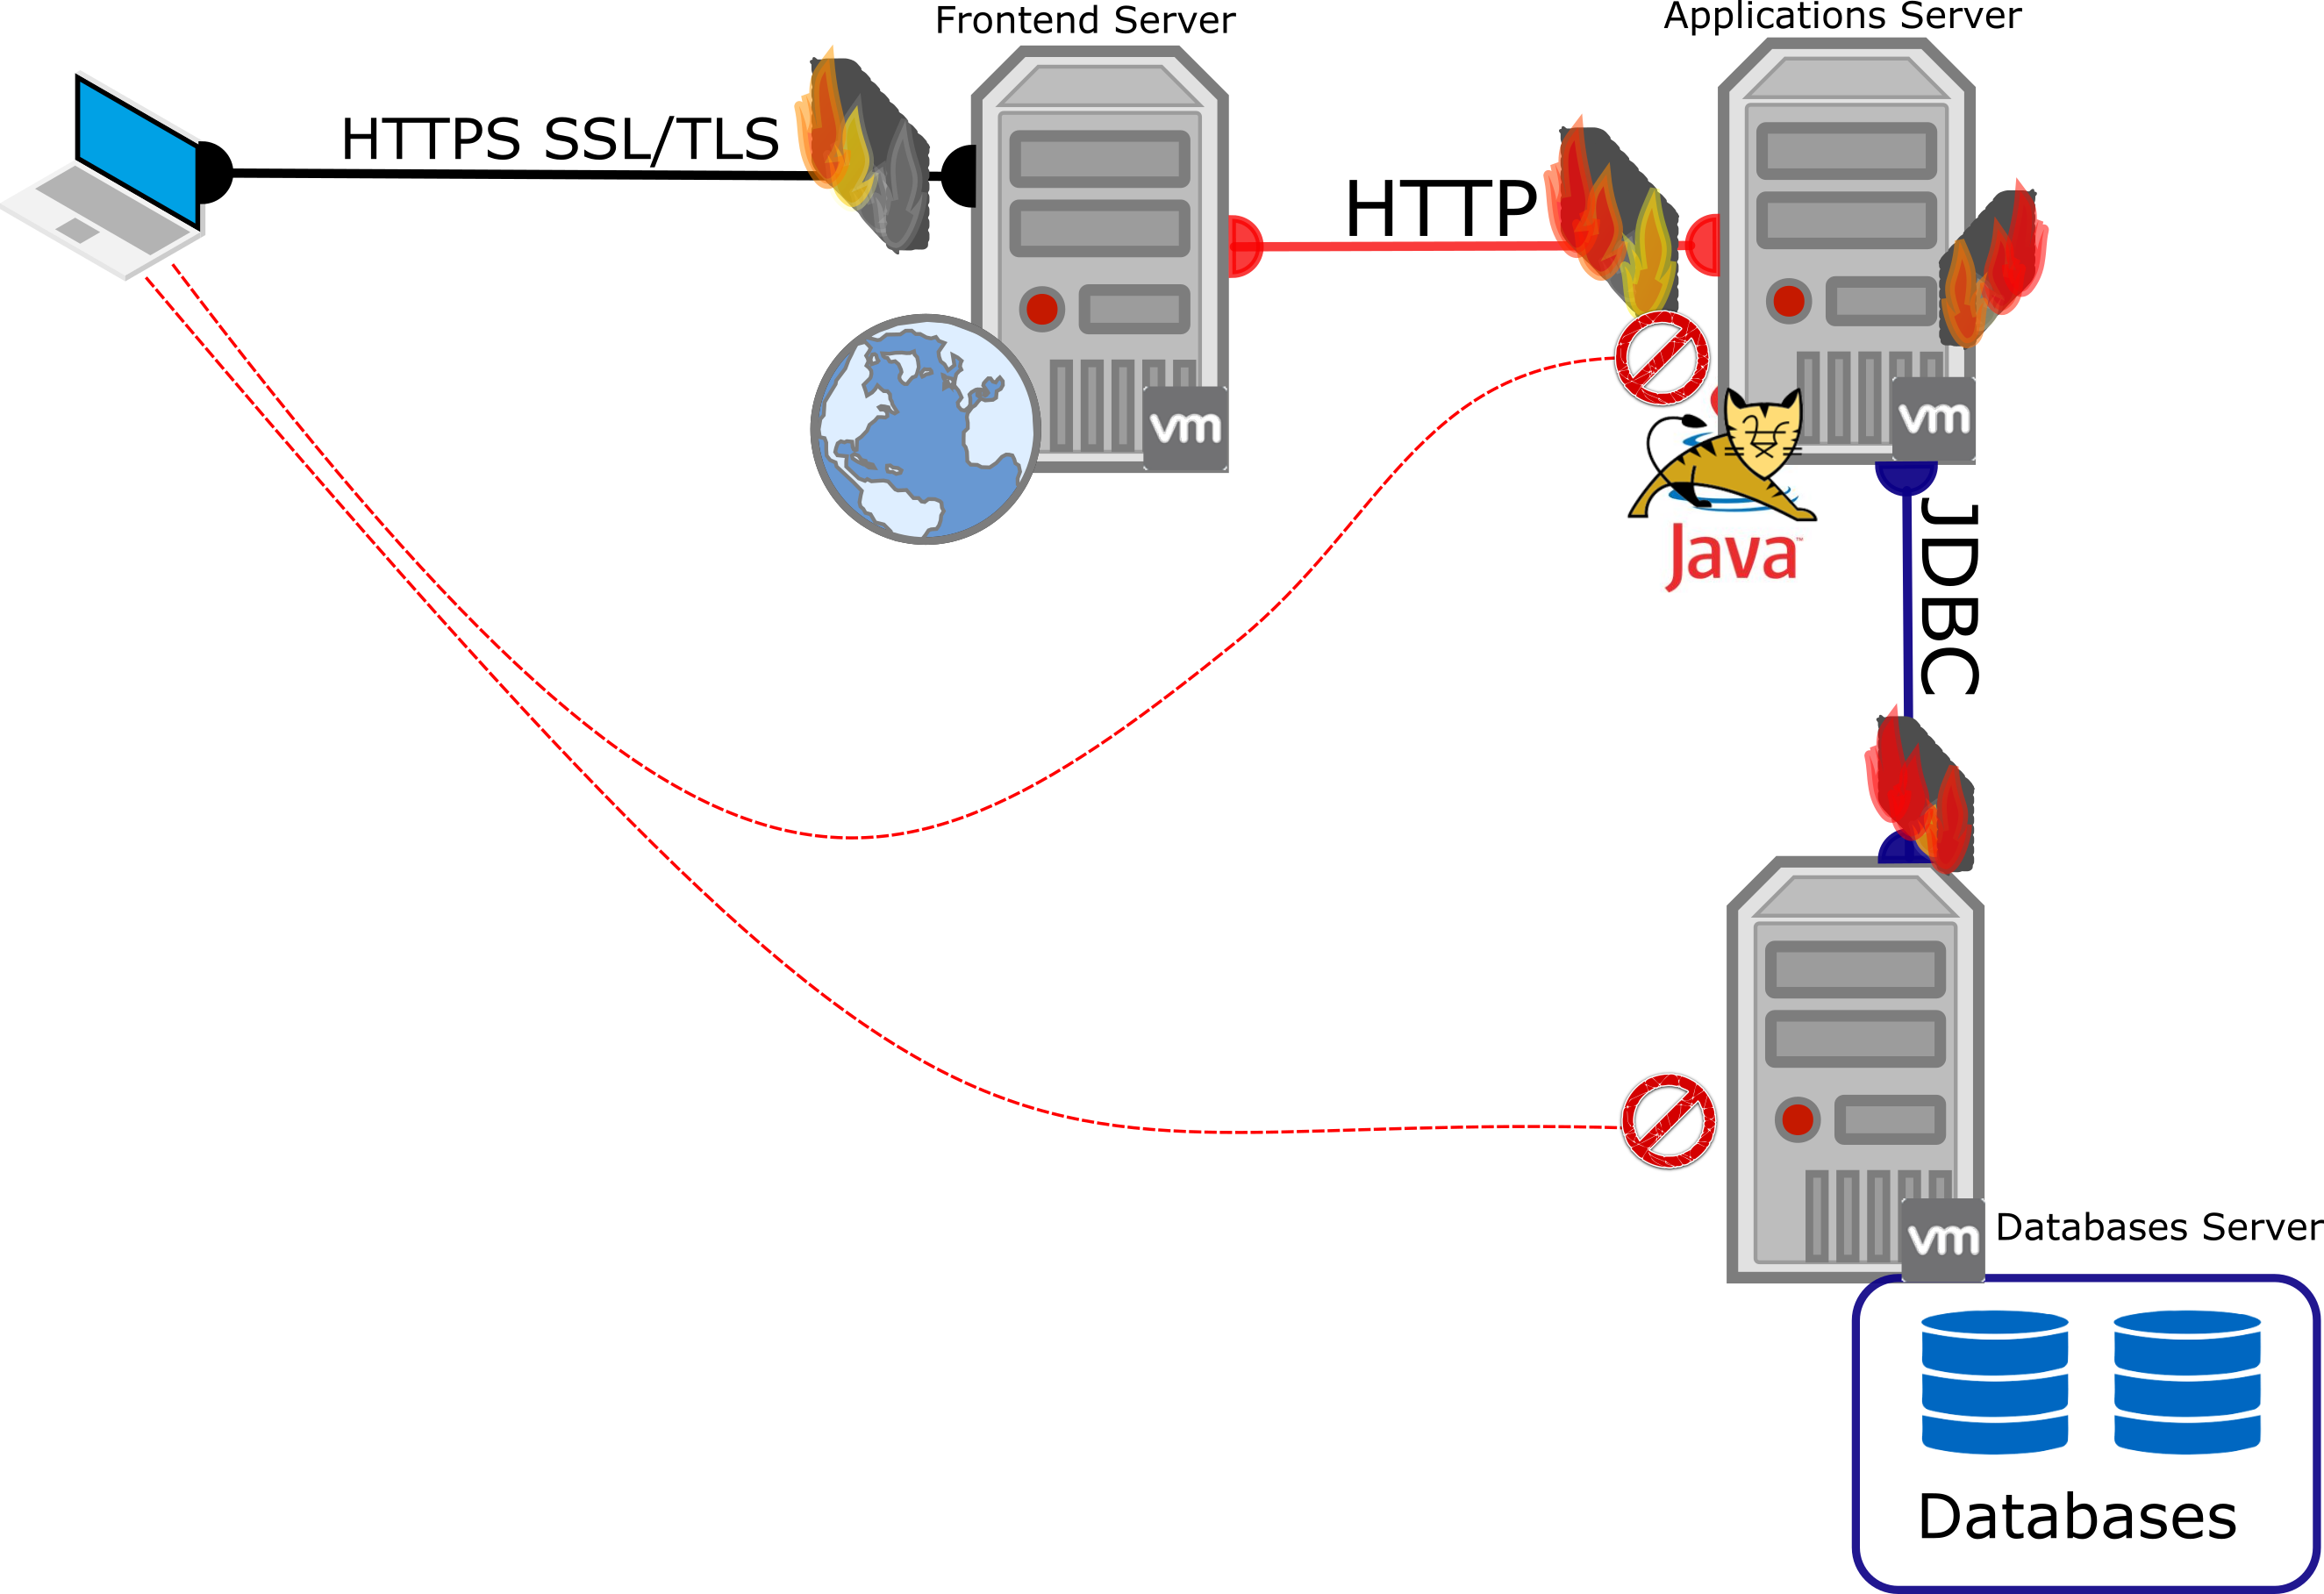
\includegraphics[scale=0.40]{./images/PNG/Application_legacy.png}
\caption{Legacy architecture}
\label{omodl}
\end{figure}

\vspace{0.5cm}

\begin{figure}[!ht]
\centering
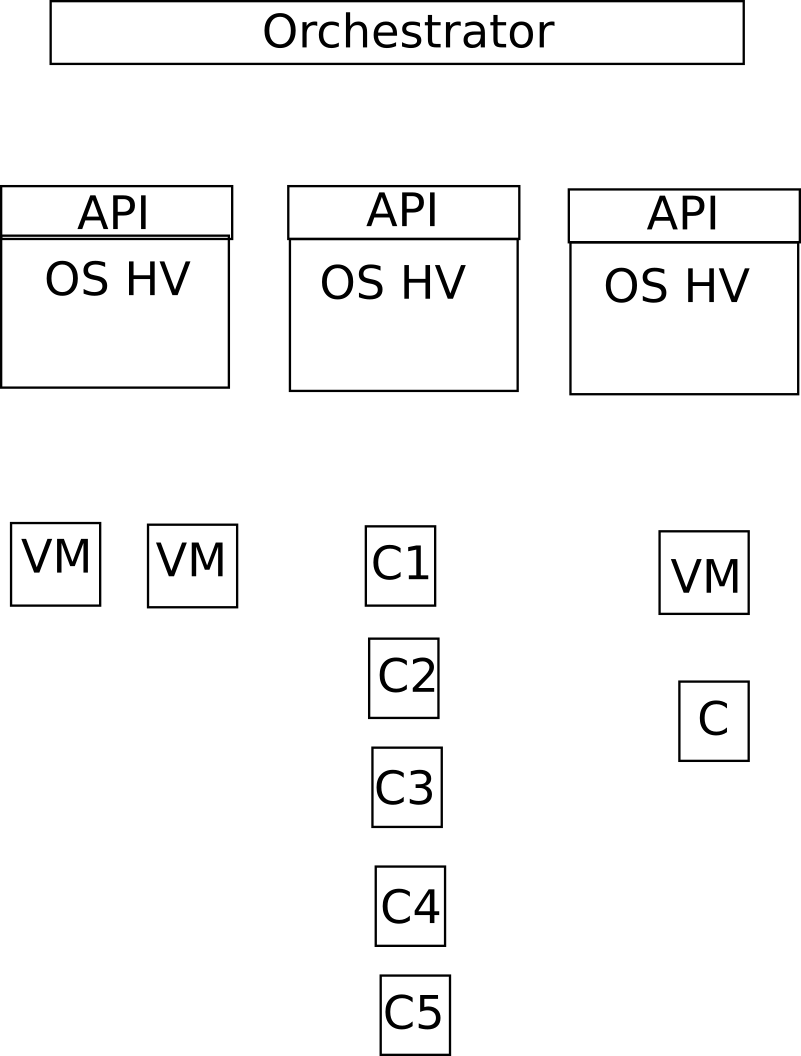
\includegraphics[scale=0.40]{./images/PNG/app2.png}
\caption{New model}
\label{nmodl}
\end{figure}


% Ok Mike

\begin{multicols}{2}
We extend here our scope of possibility to all the types of data because we need to solve the rigidity problem of the previous method. First we'll try to find a way of selecting the most influential hosts in the application i.e. the hosts for whom a variation of behavior has an important impact on the whole application. Then, we'll find a way to organize hosts into groups with common behaviors so that we can analyze the mean of the total group. Once done, we'll be able to add and remove hosts from these group without losing the learning. We expect it would also allowed more data to be used during the training of the algorithm.
\end{multicols}

\vspace{0.8cm}

\begin{multicols}{2}

\subsection{Feature selection}
\subsubsection{Signal Processing}
The signal we get from the historical data is full of small variations that may be due to measure errors or changes that are periodical parasite which are irrelevant to treat. Therefore we will try to eliminate as much noise as possible to get a better accuracy in the computation of the influence. Indeed we are going to use a correlation between signals to guess the influence of a variable over another so we have to take into account only the significant event.Furthermore we have to find a proper way of evaluating the influence a node has over another. This overview of our approach is described by Figure~\ref{trng}.
\end{multicols}

\vspace{0.8cm}

\begin{figure}[!ht]
\centering
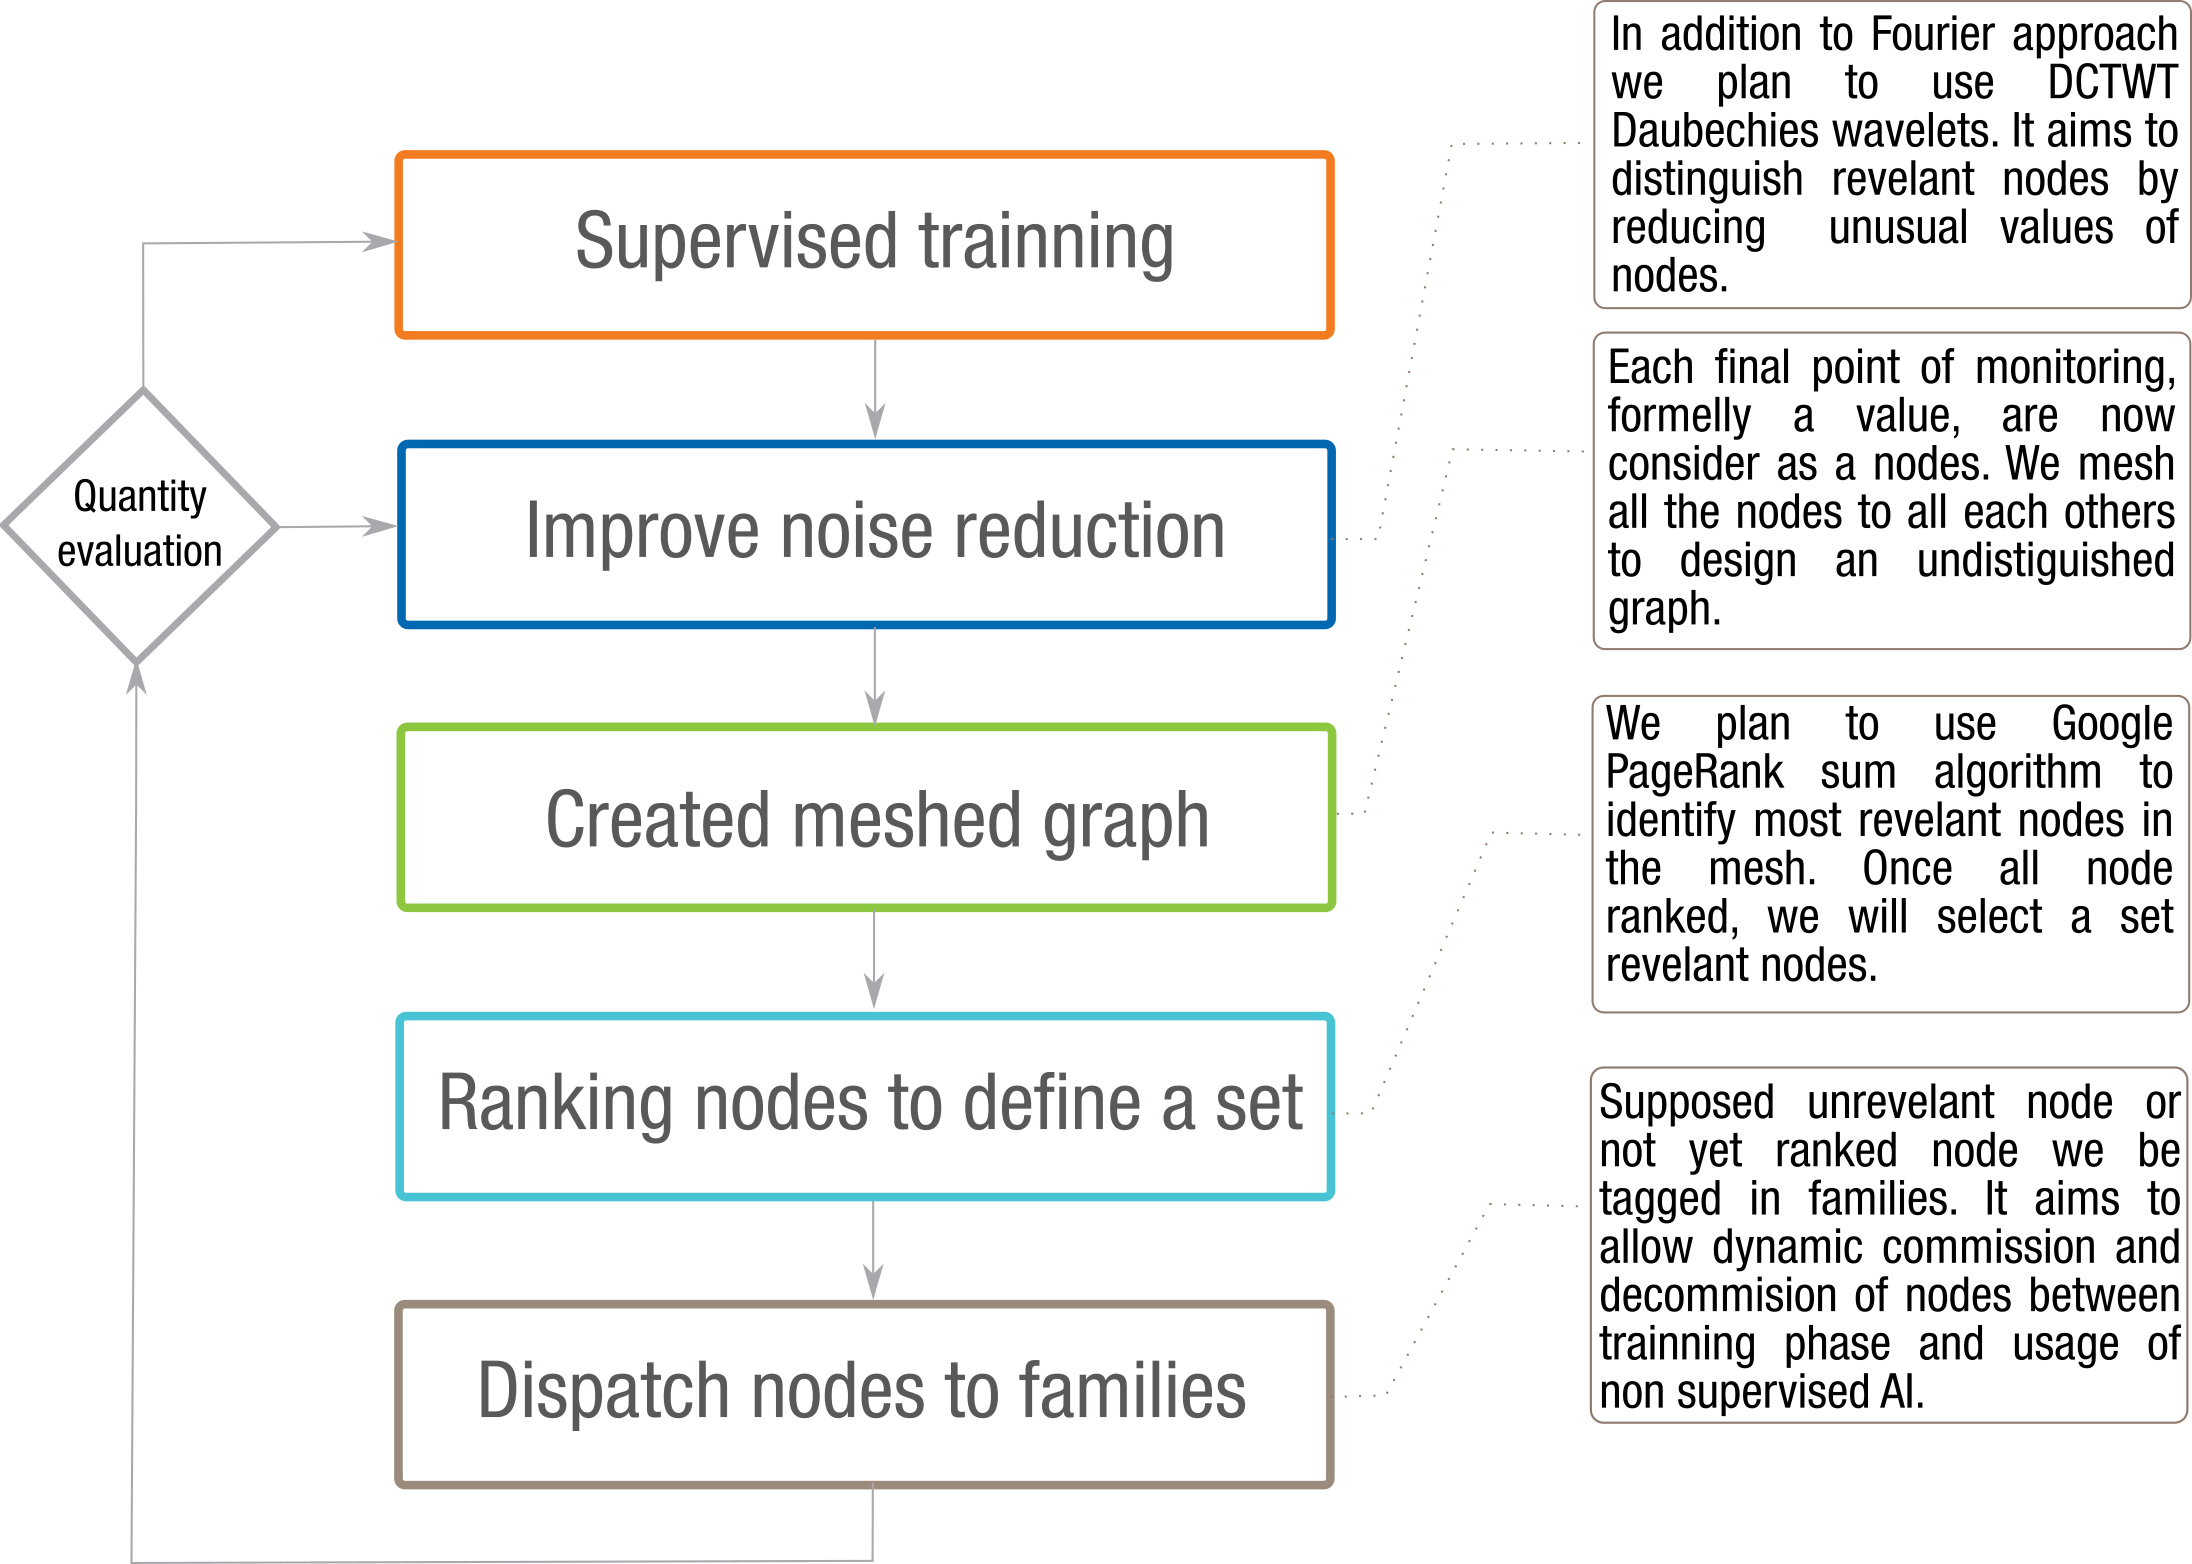
\includegraphics[scale=0.8]{./images/Apprentissage_V2.png}
\caption{Training phasing}
\label{trng}
\end{figure}

\vspace{0.8cm}

\begin{multicols}{2}
In order to reduce the noise in our signal we'll use some wavelets theory. The choosen method is described in detail in \cite{dtcwt}. Basically we transform the data in wavelet domain with DTCWT - which can be done with the dtcwt library in python for instance (see example code from the documentation below) - we then do the processing, it consists in shrinking the noisy coefficient and finally we recover the de-noised signal by doing the inverse transformation.
\end{multicols}
\begin{lstlisting}[language=Python, caption=Python dtcwt library example]
from matplotlib.pylab import *
import dtcwt


# 1D transform, 5 levels
transform = dtcwt.Transform1d()
vecs_t = transform.forward(vecs, nlevels=5)

# Inverse
vecs_recon = transform.inverse(vecs_t)
\end{lstlisting}


\begin{multicols}{2}
The transformation is a decomposition of the function into a sum of some coefficient multiplied by each vector of a family of wavelets who have specific properties (the theory is explained in detail in the paper). in this work we'll use the Daubechies' wavelets (db11 Figure~\ref{db}) which was chosen using \cite{dwtselect} and referenced papers.
\end{multicols}


\begin{figure}[!h]
\centering
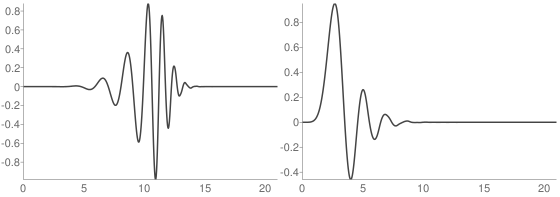
\includegraphics[scale=0.67]{./images/PNG/db11.png}
\caption{Wavelet and scaling function}
\label{db}
\end{figure}

\begin{multicols}{2}
\subsubsection{Influence evaluation}
In this part it is necessary to remember that what we are doing is done before the execution of the application during a learning phase. Therefore, we don't have any constraints in time and the algorithm can be slow.
\\
Our goal is to implement a way to evaluate the influence of each host and service on each other, we can visualize this idea as a graph where the nodes are the hosts and services and the edges are oriented. The edge $(s_i,s_j)$ is linked to the value of the influence $s_j$ has over $s_i$. As on Figure~\ref{graphe}
\end{multicols}


\begin{figure}[!h]
\centering
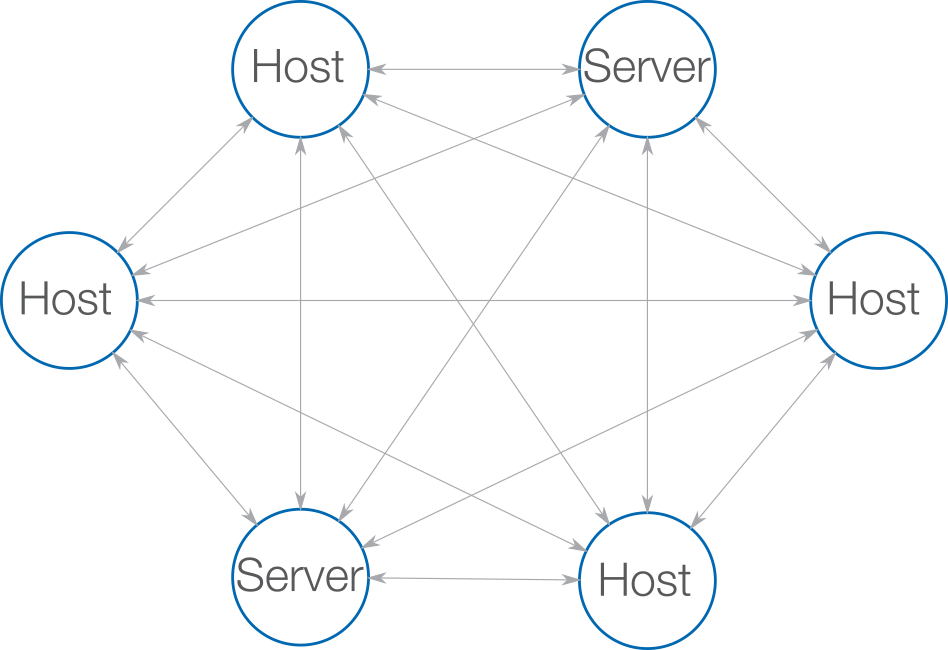
\includegraphics[scale=0.6]{./images/PNG/Graphe.png}
\caption{Graph example}
\label{graphe}
\end{figure}

%Ok Mike

\begin{multicols}{2}
The influence is assumed to be in our case the information flow between $s_i$ and $s_j$ so using the Liang-Kleeman information flow \cite{infoflow} on some data we have, we can compute the value of the edges of the graph.

\subsubsection{Targeting influential hosts}
We now want to sort the nodes by the influence they have in the graph, we'll use the principle of the $page~rank$ algorithm \cite{pagerank} on the graph where the probability to follow an edge is given by it's value of influence. this is however slightly different than the classical PageRank algorithm because edges have weights. Intuitively it can be seen as a random walk throughout the graph with the probability to follow an edge proportionnal to its weight.

To compute it however, we'll  use the power method witch is a simple and fast way to compute it. Letting $M$ the matrix of transition between the nodes, we obtain it by normalizing the scores of the edges coming out of a node and using them as probability. We compute the rank vector $X$ by starting with an arbitrary $X_0$ and then using :
	\[X_{t+1} = (dM + \frac{1-d}{N}J_N)X_t\]
until we reach :
	\[ \mid{X_t+1 - X_t}\mid < \epsilon\]
where $\epsilon$ is an arbitrarly small parameter, $N$ is the total number of nodes in the graph i.e. the number of hosts and services in the application, $J_N$ is the square matrix of size N containing only ones and finally $d$ is a parameter which represent the probability of stoping the random walk set at $0.85$ because it as been shown by experimentation done by Google that it is the optimal value to have both a decent converging rate and chance of a reaching the $X$ vector we are computing.
\end{multicols}

\begin{lstlisting}[language=Python, caption=Python Power Method]
import numpy as np

def pagerank(M, eps, d=0.85):
    N = M.shape[1]
    X = np.random.rand(N, 1)
    X = X / np.linalg.norm(X, 1)
    X_{t-1} = np.ones((N, 1), dtype=np.float32) * np.inf
    T = (d * M) + (((1 - d) / N) * np.ones((N, N), dtype=np.float32))
    
    while np.linalg.norm(X - X_{t-1}, 2) > eps: 
        X_{t-1} = X
        X = np.matmul(T, X)
    return X

\end{lstlisting}



\begin{figure}[!h]
\centering
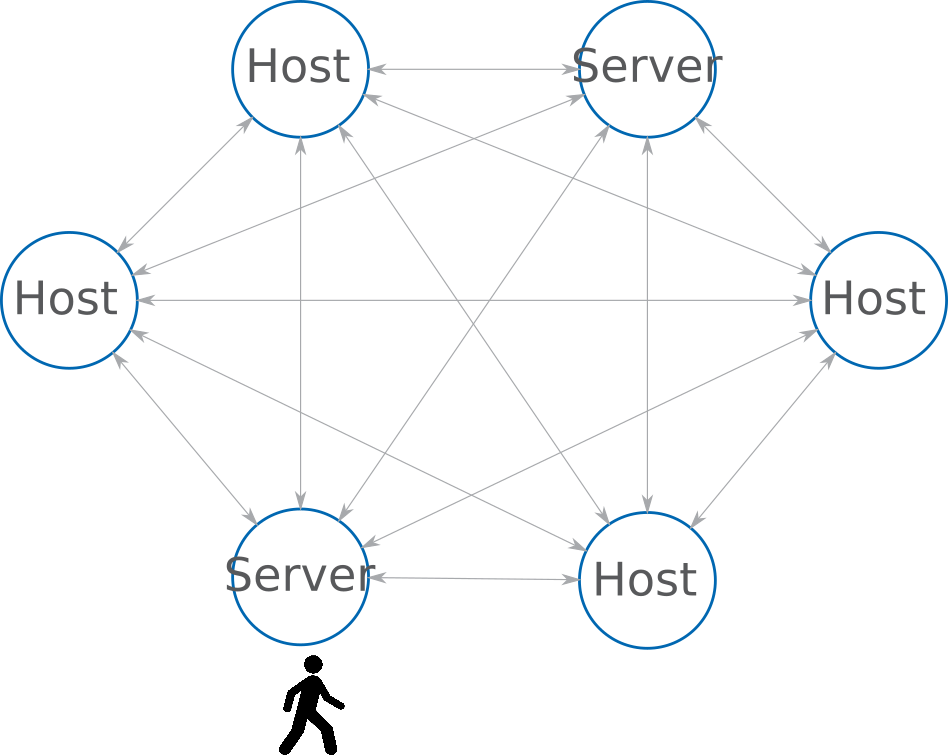
\includegraphics[scale=0.5]{./images/PNG/GraphesRandomWalk.png}
\caption{Random walk : initial state}
\label{graphrwb}
\end{figure}

\begin{figure}[!h]
\centering
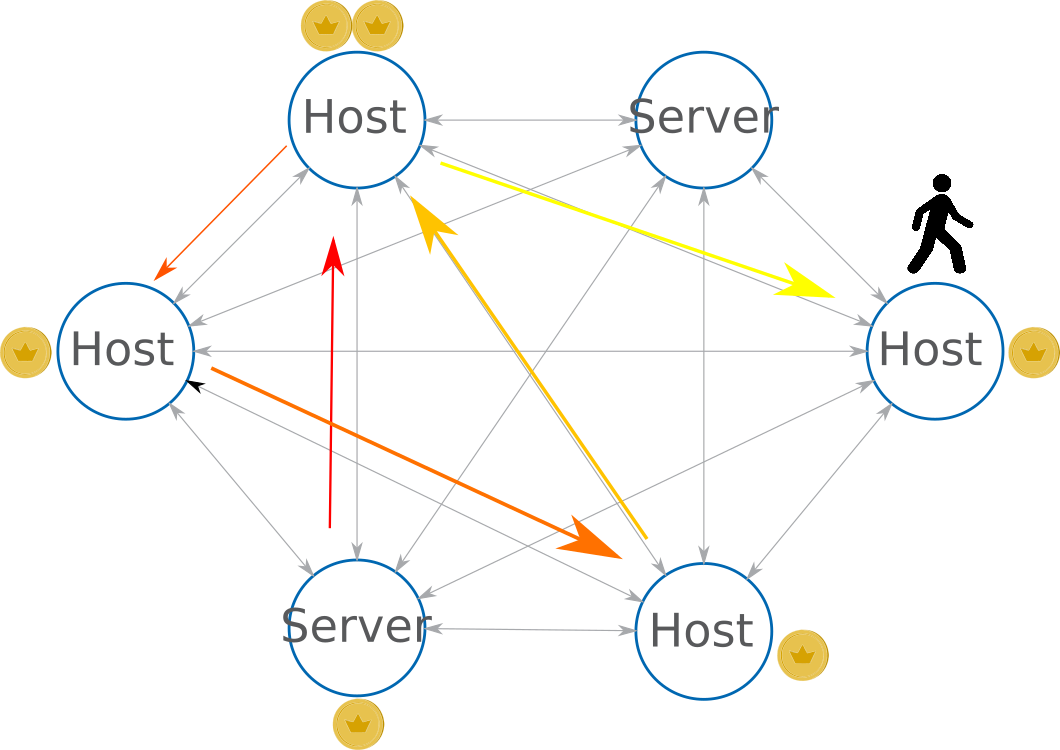
\includegraphics[scale=0.5]{./images/PNG/GraphesRandomWalk2.png}
\caption{Random walk : advanced state}
\label{graphrw}
\end{figure}


\begin{multicols}{2}
\subsubsection{Conclusion}
Using these different techniques we manage to get a subset of all the hosts and services which are the one with most influence on the whole application. We can focus our learning on these particular variables. Which means that we'll have to deal with architectural changes of the application less often, beside it should also lighten the computations during the training phase. However we'll try to get some more information by grouping the other variables together insuring the flexibility of the application and light computations.\\
\subsection{Grouping features}
Finally when we selected our principal features we cluster all the others in order to be able to adapt to changes in the application architecture. We assumed that the variables that will be removed and added the most often also have limited impact on the global application.\\
We'll use the nearest neighbors process clustering described in this article \cite{ref5} (which also expose a K mean algorithm but this one is said to be less effective with small amount of data, which may be the case in our situation) and then we'll use the method described in the first part on the selcted features and a mean of the ones in each cluster.



\end{multicols}

\vspace{0.8cm}

\bibliographystyle{plain} 
\begin{thebibliography}{9}
    \bibitem{dwtselect}
      Nick Kingsbury,
      \emph{SHIFT INVARIANT PROPERTIES OF THE DUAL-TREE COMPLEX WAVELET TRANSFORM}.
        \\\texttt{https://pdfs.semanticscholar.org/9da5/3dc0ef012916ba9955698451231fdc0d2890.pdf}

    \bibitem{dtcwt2}
      2 R.K Sarawale and Dr S.R Chougule,
      \emph{Image Denoising using Dual-Tree Complex DWT and Double-Density Dual-Tree Complex DWT}.
        \\\texttt{https://pdfs.semanticscholar.org/ca23/05f7bb9caa189200abe2c4ad403bc8759ecc.pdf}

    \bibitem{infoflow}
      X. San Liang,
      \emph{The Liang-Kleeman Information Flow: Theory and Applications}.
        \\\texttt{https://pdfs.semanticscholar.org/c3ba/9dc7452d88ae8e88f7e651442ae3e5c039cb.pdf}
        
    \bibitem{pagerank}
      Sergey Brin and Lawrence Page,
      \emph{The Anatomy of a Large-Scale Hypertextual Web Search Engine}.
        \\\texttt{http://infolab.stanford.edu/pub/papers/google.pdf}

        
\end{thebibliography}

\vspace{0.8cm}
Main author: Chanus Baptiste - Coordinator Aubertin Michael\\
Contact: maubertin@fr.scc.com

\end{document}

